\chapter{Enjeux}
\section{Descriptif de la smart grid}

% Smart grid

La smart grid est l'union de deux expertises, l'informatique et l'énergie.
Ce type réseau permet l'échange d'informations sur l'état du réseau.
Ces connaissances sont importantes pour pouvoir optimiser la distribution, faire du stockage
ainsi que l'impacte écologique de l'homme.

L'un des intérêts de ce partage d'information est de pouvoir décentraliser la production d'énergie,
ainsi, tout point du réseau peut produire ou consommer son energie.
Cette complexité supplémentaire nécessite de nombreux ajustements et changements de paradigme.
L'un de ces changement est le coût de l'énergie, celle-ci varie déjà aujourd’hui, mais cette variation
devrait être d'autant plus importante que les énergies renouvelables prendront une place forte dans
le mix énergétique citadin. Une solution serait que chaque ville possède une bourse de l'énergie
locale qui atténuerait les variations, et profiterait aux personnes consommant en heures creuses.

\begin{SCfigure}[][h]
    \centering
    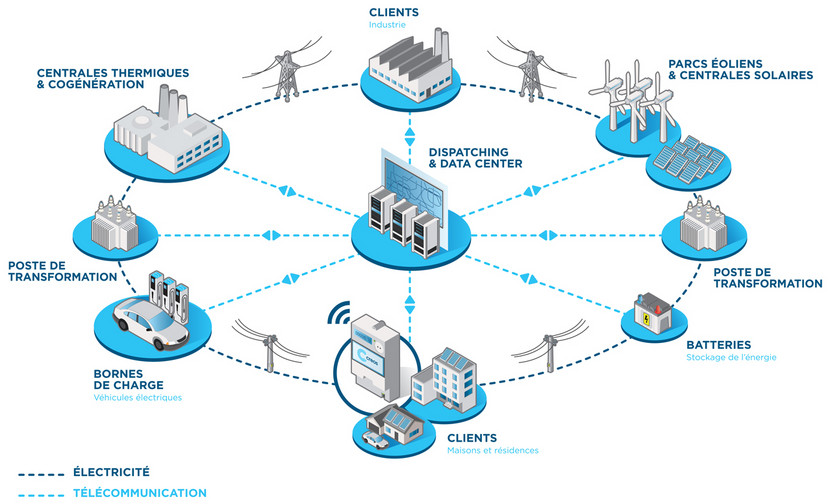
\includegraphics[scale=0.25]{media/smart_city_lux.jpg}
    \caption{
        Architecture d'une smartgrid\newline
        \tiny{Source: \url{https://www.creos-net.lu/creos-luxembourg/innovation/smart-grid/reseau-du-futur.html}}
    }
\end{SCfigure}

% Micro grid

La microgrid est un autre type de réseau qui, contrairement à la smart grid, ne s'occupe pas de la communication.
Cette solution est envisagée plus sérieusement par de nombreuses communes pour des raisons de coût, en effet, ses
avantages restent nombreux tels que la gestion de différentes sources d'énergies opérée de manière parallèle,
ainsi qu'une fiabilisation du réseau déjà présent.

% https://www.researchgate.net/post/What_is_the_difference_between_a_microgrid_and_a_smartgrid
% A microgrid is an electrical system that includes multiple loads and distributed energy resources that can be operated in parallel with the
% broader utility grid or a Small, independent power system. It Increased reliability with distributed generation, Increase efficiency
% with reduced transmission length, and Easier integration of alternative energy sources.while
% A smart grid is a modernized electrical grid that uses information and communications technology to gather and act on information,
% such as information about the behaviors of suppliers and consumers, in an automated fashion to improve the efficiency, reliability,
% economics, and sustainability of the production and distribution of electricity. Transmission and operations: wide‐area monitoring,
% control and protection.


% Analyse des villes

\section{Villes connectées}
% Cette partie parlera de la partie technique de la mise en place de la smart grid
%   Ainsi que des différents problèmes que les villes actuelles ont.

\section{Connectivité et population}
% Cette partie parlera de la partie humaine de la connexion a la smart grid.
% ex. La 5G (6G) et les réseaux sociaux
%     Communication et report de problèmes

\section{Les mutations de la ville}



\section{Étude de cas - IssyGrid}
Le projet IssyGrid® a été initié en 2012 par Bouygues Immobilier dans la ville d'Issy-les-Moulineaux,
commune française dans le département des Hauts-de-Seine. Le projet a été fortement encouragé par le
maire de la commune, André Santini. Mais aucun soutien d'ordre financier.

``La ville n’a pas mis un euro'' --  Éric Legale, directeur d’IssyMedia, chargé de la communication et
de l’innovation de la ville.

Le projet n'a pas impliqué qu'un seul acteur, mais un consortium de dix compagnies :
Bouygues Energies \& Services, Bouygues Immobilier, Bouygues Telecom, EDF, EMBIX, Enedis,
Microsoft, Schneider Electric, Sopra Steria et Total.

L'expérience a duré 6 ans, de 2012 à 2018, et a un impact sur la vie de 5.000 habitants, 10.000 employés
et 160.000 m2 de bureaux sur deux quartiers de la ville, Bords-de-Seine (quartier des affaires),
puis Fort en 2015.

Le projet a fait face à plusieurs types de défis. Tout d'abord des défis techniques.

Les habitations concernées ont été équipées d'un Linky, un compteur électrique conçu par EDF
plus intelligent que les anciens. Il est capable de suivre et de communiquer la consommation en
électricité tout comme son cousin Gazpar pour la consommation de gaz. La création de ces appareils répond
à une directive européenne, mais ils ont utiliser les Eco-quartiers comme terrain de test.
Total a également fait des progrès sur le raccordement des panneaux photovoltaïques.
L'énergie créée en trop lors des heures creuses est stockée dans des volants d'inertie et dans des
batteries. un accord a été passé avec Renault pour récupérer leurs anciennes batteries de voitures
électriques, démontrées comme suffisantes pour les quartiers Isséens.
Bouygues Energies \& Services a également travaillé sur l'éclairage urbain pour que les réverbères
consomment moins d'énergie et lutter contre la pollution lumineuse. Ils sont capables d'adapter
leur éclairage en fonction de l'heure et des présences à proximité.
Les données transitent dans toute la Smart Grid au travers d'un réseau développé par Embix, une
start-up créée par Bouygues. Ils ont livré le centre d'analyse et d'optimisation de l'ensemble des
flux énergétique, capable de communiquer avec tous les instruments de mesure du quartier, avec autant de
protocoles différents.

Mais aussi un défi concernant la récolte et l'utilisation des données utilisateurs.

Les informations de consommation d'énergie et de déplacements sont essentielles pour que la ville
puisse s'adapter à sa population. Le projet est parvenu à un accord sans précédent avec la CNIL :
la collecte des données est autorisée par lot de dix habitations afin de la garder anonyme, garantir
la confidentialité particulière d'un logement.
D'autant plus que la ville a choisi de faire de l'Open Data. Chaque foyer doit toutefois
donner son accord pour que ses données alimente le flux.

Un autre défi majeur fut la communication.

Tout au long du projet, la ville a fait un éffort de vulgarisation du projet afin de rassurer
la population par divers moyens de communication et de modules pédagogiques. La population a accès
a une interface pour suivre la consommation et la production d'énergie en temps réel grâce à des
graphes simples et intuitifs afin de la sensibiliser et la rendre actrice du projet.

Le projet IssyGrid inclus deux autres projets : SWAYS et SoMobility.

SWAYS - Smart ways to work - est un immeuble de travail de l'éco-quartier des affaires de IssyGrid.
Tout est fait pour le améliorer le confort des utilisateurs.
Il privilégie un éclairage naturel dans les bureaux et la purification de l'air par la biophilie,
le tout grâce à un toit végétale. Des commerces de proximité et autres structures de loisir
sont installés à l'intérieur même du bâtiment. D'un point de vue technique, le bâtiment serait
capable de d'anticiper les pannes grâce à de la maintenance prédictive, assure une couverture réseau
4G dans tout le complexe, et propose même aux utilisateurs des applications liées à l'activité du
bâtiment, ainsi qu'une cyber sécurité renforcée.

SoMobility est un projet dont le but est de fluidifier la circulation dans la ville. Les feux de
signalisation sont par exemple capables de prendre des initiatives pour optimiser le trafic.
Des applications proposent aux utilisateurs d'indiquer les places de parkings libres sur une carte.
Il y a actuellement un mini-bus qui se déplace sans chauffeur dans la ville.
Les données de circulation de ma ville sont encore une fois open data. Il est possible de visualiser
le trafic en temps réel sur plusieurs sites internet.
Au delà des ressources techniques mise en place, les habitants sont aussi sensibilisés à travailler
dans des espaces de coworking avant d'aller au bureau afin de désengorger les routes et transports
en commun, et le covoiturage est aussi mis en avant.

Le bilan de IssyGrid a été présenté en juin 2019.
Il ne présente malheureusement pas de chiffres pour ces six années de test, mais annonce en revanche
ses objectifs pour 2020 : ``Une efficacité énergétique accrue de 20 \%, une réduction de 20 \%
de l’empreinte carbone et une part de 20 \% des énergies renouvelables dans la production
énergétique européenne.''
La ville d'Issy-les-Moulineaux souhaite agrandir la Smart Grid à un troisième quartier
``Issy Coeur de Ville''. La ville de Nanterre s'inspire de ce projet pour lancer un projet
d'éco-quartier également.
Les chiffres d'IssyGrid n'ont pas été communiqués, mais un témoignage de Gironde HABITAT nous indique
que l'économie générée sur la consommation énergétique serait au mieux de 60€ par an à l'échelle d'un
foyer.

Questions pour la ville d'Issy les Moulineaux :
\begin{itemize}
    \item Le projet a été initié par Bouygues. Comment on été réparties les missions entre toutes les entreprises du
consortium et la ville ?
    \item Comment a été financé le projet ? Combien a été investi dedans ?
    \item Quels projets de smart grid avez vous pu analyser lors de la réflexion du projet IssyGrid ?
    \item Quels sont les enseignements que vous en avez tiré ? Quels éléments auraient pu mettre le projet
en échec ? Quels étaient les quick win ?
    \item Y a t il eut des oppositions au projet de la part des Isséens ? Comment ces conflits ont ils été réglé ?
    \item Où est ce que les isséens peuvent voir la consommation de la ville en temps réel ?
    \item Quels sont les prochains projets pour la ville et comment avancent-ils ?
    \item Les quartiers impactés par IssyGrid ont-ils pris de la valeur ou sont-ils accessibles
au même prix par la population ?
    \item Quelles sont les économies en énergie réalisées par un foyer par an ?
    \item Pourquoi des panneaux photovoltaïque et pas des turbines éoliennes sur le toit des immeubles ?
\end{itemize}

Questions pour EMBIX :
\begin{itemize}
    \item Comment circule le flux de données dans la grid ? Les informations sont-elles stockées sur un serveur distants,
sont-elles diffusées grâce à du peer-to-peer ?
    \item Avez-vous calculé l'emprunte carbone de IssyGrid ? Si oui, quel est-il ? Sauriez-vous le comparer avec l'emprunte
carbone avant le début du projet ?
    \item Quels sont vos futurs projets ambitieux en terme d'éco-quartier ?
    \item De quels types de capteur la ville Issy les Moulineaux est elle équipée ?
\end{itemize}


\section{Des projets en échec}

Lors de la VivaTech Paris 2019, Emmanuel BAVIERE (Société Générale), Erwan KERYER (KPMG)
et Jérôme MONCEAUX (SPOON) ont pris la parole le vendredi 16 mai pour expliquer le phénomène autour des
Smart Grid. Un terme fort a été employé durant cette prise de parole :
``La Smart City ne marche pas''.

En se basant sur plusieurs exemples de projets en échec, divers arguments à ce propos ont été mis en
avant :
\begin{itemize}
    \item Des projets trop ambitieux ;
    \item Un manque de communication avec la population qui fait face à une puissance effrayante car mal comprise ;
    \item Les grands groupes ne savent pas comment gérer les tensions et désaccords avec les élus et la population ;
    \item Un manque de formation de la population qui ne sait pas utiliser les nouvelles technologies ;
    \item Une population qui refuse de partager ses données pourtant nécessaires au bon fonctionnement d’une Smart Grid ;
    \item Le gouffre séparant les populations aisées des populations pauvres s'élargie.
\end{itemize}

Le projet Quayside de Toronto réunit la plupart de ces éléments.
% Description du projet
Les oppositions au projet sont multiple. On lui reproche avant tout son manque de démocratie.
Bianca Wylie, une opposante au projet, accuse les grands groupes derrière le projet de vouloir noyer l'information
avec la publication d'un document aussi volumineux auprès de la population.